% !TEX TS-program = lualatex
% !TEX encoding = UTF-8 Unicode
\documentclass[12pt,a4paper]{article}

\IfFileExists{src/libs/body.tex}{% --- body.tex ---
\usepackage{pdfpages}
\usepackage{fontspec}
% Prefer Times New Roman when available; fall back in container environments.
\IfFontExistsTF{Times New Roman}{
  \setmainfont{Times New Roman}
}{
  \setmainfont{Liberation Serif}
}
\usepackage[vietnamese]{babel}

% Page layout and spacing
\usepackage[left=3cm,right=2cm,top=2cm,bottom=2cm]{geometry}
\usepackage{titlesec}
\usepackage{setspace}

% Silence noisy warnings
\usepackage{silence}
\WarningFilter{transparent}{Loading aborted}
\WarningFilter{hyperref}{The anchor of a bookmark and its parent's}

% Core packages
\usepackage{float}
\usepackage{svg}
\usepackage{graphicx}
\graphicspath{{assets/}{../assets/}{../../assets/}}
\svgpath{{assets/}{../assets/}{../../assets/}}
\usepackage{enumitem}
\usepackage{array}
\usepackage{tabularx}
\usepackage{multirow}
\usepackage[table]{xcolor}
\usepackage{ulem}
\usepackage{xurl}

% ====== THÊM 2 GÓI NÀY ĐỂ FIX LỖI ADJUSTBOX VÀ FOREST ======
\usepackage{adjustbox}
\usepackage[edges]{forest}
% ============================================================

% TikZ
\usepackage{tikz}

% ====== BỔ SUNG FIT, BACKGROUNDS, TREES VÀO DANH SÁCH ======
\usetikzlibrary{calc, arrows.meta, shapes.geometric, positioning, fit, backgrounds, trees}

% Table tuning
\renewcommand{\tabularxcolumn}[1]{m{#1}}
\hbadness=10000
\hfuzz=10000pt

% Shared commands
\newcommand{\subsecheading}[1]{%
    \par\vspace{2pt}%
    \hspace{1.5em}\textbf{#1}%
    \par\vspace{2pt}%
}
\newcommand{\introtext}[1]{%
    \par\hspace{3.0em}#1\par%
}
\newcommand{\StandaloneDocumentSetup}[2]{%
  \pagenumbering{arabic}%
  \ApplyStandardFooter{#1}{#2}%
}
\newcommand{\StandaloneSectionSetup}[2]{%
  \ApplyStandardFooter{#1}{#2}%
}

% Math
\usepackage{amsmath}

% Hyperref
\usepackage{hyperref}
\hypersetup{
    colorlinks=true,
    linkcolor=black,
    filecolor=magenta,
    urlcolor=blue,
}}{% --- body.tex ---
\usepackage{pdfpages}
\usepackage{fontspec}
% Prefer Times New Roman when available; fall back in container environments.
\IfFontExistsTF{Times New Roman}{
  \setmainfont{Times New Roman}
}{
  \setmainfont{Liberation Serif}
}
\usepackage[vietnamese]{babel}

% Page layout and spacing
\usepackage[left=3cm,right=2cm,top=2cm,bottom=2cm]{geometry}
\usepackage{titlesec}
\usepackage{setspace}

% Silence noisy warnings
\usepackage{silence}
\WarningFilter{transparent}{Loading aborted}
\WarningFilter{hyperref}{The anchor of a bookmark and its parent's}

% Core packages
\usepackage{float}
\usepackage{svg}
\usepackage{graphicx}
\graphicspath{{assets/}{../assets/}{../../assets/}}
\svgpath{{assets/}{../assets/}{../../assets/}}
\usepackage{enumitem}
\usepackage{array}
\usepackage{tabularx}
\usepackage{multirow}
\usepackage[table]{xcolor}
\usepackage{ulem}
\usepackage{xurl}

% ====== THÊM 2 GÓI NÀY ĐỂ FIX LỖI ADJUSTBOX VÀ FOREST ======
\usepackage{adjustbox}
\usepackage[edges]{forest}
% ============================================================

% TikZ
\usepackage{tikz}

% ====== BỔ SUNG FIT, BACKGROUNDS, TREES VÀO DANH SÁCH ======
\usetikzlibrary{calc, arrows.meta, shapes.geometric, positioning, fit, backgrounds, trees}

% Table tuning
\renewcommand{\tabularxcolumn}[1]{m{#1}}
\hbadness=10000
\hfuzz=10000pt

% Shared commands
\newcommand{\subsecheading}[1]{%
    \par\vspace{2pt}%
    \hspace{1.5em}\textbf{#1}%
    \par\vspace{2pt}%
}
\newcommand{\introtext}[1]{%
    \par\hspace{3.0em}#1\par%
}
\newcommand{\StandaloneDocumentSetup}[2]{%
  \pagenumbering{arabic}%
  \ApplyStandardFooter{#1}{#2}%
}
\newcommand{\StandaloneSectionSetup}[2]{%
  \ApplyStandardFooter{#1}{#2}%
}

% Math
\usepackage{amsmath}

% Hyperref
\usepackage{hyperref}
\hypersetup{
    colorlinks=true,
    linkcolor=black,
    filecolor=magenta,
    urlcolor=blue,
}}
\IfFileExists{src/libs/header.tex}{% --- header.tex ---
\usepackage{fancyhdr}
\setlength{\headheight}{15.5pt} % Thêm dòng này để fix cảnh báo chiều cao
%\setlength{\headheight}{14.5pt}
\addtolength{\topmargin}{-2.5pt}

\pagestyle{fancy}
\fancyhf{}
\renewcommand{\headrulewidth}{0pt}
\renewcommand{\footrulewidth}{0pt}

\newcommand{\ApplyStandardHeader}{%
  \fancyhead[L]{%
    \begin{minipage}[t]{0.795\linewidth}%
      UIT \textbar{} SS004.F21 \textbar{} Nhóm 03 \textbar{} Đồ án cuối kỳ%
    \end{minipage}%
    \vrule%
    \begin{minipage}[t]{0.185\linewidth}%
      \centering cTetris%
    \end{minipage}%
  }%
}

\ApplyStandardHeader
}{% --- header.tex ---
\usepackage{fancyhdr}
\setlength{\headheight}{15.5pt} % Thêm dòng này để fix cảnh báo chiều cao
%\setlength{\headheight}{14.5pt}
\addtolength{\topmargin}{-2.5pt}

\pagestyle{fancy}
\fancyhf{}
\renewcommand{\headrulewidth}{0pt}
\renewcommand{\footrulewidth}{0pt}

\newcommand{\ApplyStandardHeader}{%
  \fancyhead[L]{%
    \begin{minipage}[t]{0.795\linewidth}%
      UIT \textbar{} SS004.F21 \textbar{} Nhóm 03 \textbar{} Đồ án cuối kỳ%
    \end{minipage}%
    \vrule%
    \begin{minipage}[t]{0.185\linewidth}%
      \centering cTetris%
    \end{minipage}%
  }%
}

\ApplyStandardHeader
}
\IfFileExists{src/libs/footer.tex}{% --- footer.tex ---
\usepackage{lastpage}

\newcommand{\ApplyStandardFooter}[2]{%
  \fancyfoot[L]{%
    \begin{minipage}[t]{0.795\linewidth}%
      Document ID: #1%
    \end{minipage}%
    \vrule%
    \begin{minipage}[t]{0.185\linewidth}%
      \centering\thepage/\pageref{#2}%
    \end{minipage}%
  }%
  \fancypagestyle{plain}{%
    \fancyhf{}%
    \renewcommand{\headrulewidth}{0pt}%
    \renewcommand{\footrulewidth}{0pt}%
    \ApplyStandardHeader%
    \fancyfoot[L]{%
      \begin{minipage}[t]{0.795\linewidth}%
        Document ID: #1%
      \end{minipage}%
      \vrule%
      \begin{minipage}[t]{0.185\linewidth}%
        \centering\thepage/\pageref{#2}%
      \end{minipage}%
    }%
  }%
  \pagestyle{fancy}%
}
}{% --- footer.tex ---
\usepackage{lastpage}

\newcommand{\ApplyStandardFooter}[2]{%
  \fancyfoot[L]{%
    \begin{minipage}[t]{0.795\linewidth}%
      Document ID: #1%
    \end{minipage}%
    \vrule%
    \begin{minipage}[t]{0.185\linewidth}%
      \centering\thepage/\pageref{#2}%
    \end{minipage}%
  }%
  \fancypagestyle{plain}{%
    \fancyhf{}%
    \renewcommand{\headrulewidth}{0pt}%
    \renewcommand{\footrulewidth}{0pt}%
    \ApplyStandardHeader%
    \fancyfoot[L]{%
      \begin{minipage}[t]{0.795\linewidth}%
        Document ID: #1%
      \end{minipage}%
      \vrule%
      \begin{minipage}[t]{0.185\linewidth}%
        \centering\thepage/\pageref{#2}%
      \end{minipage}%
    }%
  }%
  \pagestyle{fancy}%
}
}
\usepackage{docmute}
\usepackage{tabularx}
\usepackage{enumitem}
\usepackage{booktabs}
\usepackage{multirow}
\usepackage{colortbl}
\usepackage{tikz}
\usetikzlibrary{shapes.geometric,arrows.meta,positioning,calc,fit,backgrounds}

\definecolor{v1green}{RGB}{20,130,80}
\definecolor{v2amber}{RGB}{190,120,10}
\definecolor{v3red}{RGB}{170,40,40}
\definecolor{storyBlue}{RGB}{30,90,200}
\definecolor{consoleOrange}{RGB}{200,100,20}
\definecolor{coreViolet}{RGB}{100,30,160}
\definecolor{headerGray}{RGB}{60,60,60}
\definecolor{rowLight}{RGB}{245,247,250}

\hypersetup{pdftitle={WBS \& Effort Estimation -- cTetris Project}}

\begin{document}
\providecommand{\StandaloneSectionSetup}[2]{\ApplyStandardFooter{#1}{#2}}
\StandaloneSectionSetup{13-projectEffortEstimation.tex}{LastPageProjectEffortEstimation}
\onehalfspacing

% ══════════════════════════════════════════════════════════════════
\section{Ước Tính Công Sức \& Phân Rã Công Việc (WBS)}
% ══════════════════════════════════════════════════════════════════

\subsection{Khung Phương Pháp (Estimation Framework)}

Dự án \textbf{cTetris} áp dụng mô hình phân rã ba tầng để định lượng công sức đầu tư, đảm bảo tính minh bạch từ mức chi tiết nhỏ nhất (hàm/tính năng đơn lẻ) đến mức tổng hợp toàn dự án.
\subsubsection{Mô hình Ba Tầng (Three-Tier Model)}

\begin{center}
\begin{tikzpicture}[
  tier/.style={rectangle,rounded corners=4pt,draw=headerGray,fill=rowLight,
               minimum width=11cm,minimum height=0.75cm,align=center,font=\small},
  label/.style={font=\footnotesize\itshape,text=gray},
  arrow/.style={-{Stealth[length=5pt]},thick,gray}
]
  \node[tier,fill=v3red!10,draw=v3red](t3) at (0,0)
    {\textbf{Tầng 3 — Phiên bản Module (Module Version)}
     \quad\footnotesize Tập hợp nhiều Big Tasks + Independent Small Tasks (fixes/prep)};
\node[tier,fill=v2amber!10,draw=v2amber,below=0.4cm of t3](t2)
    {\textbf{Tầng 2 — Thành phần (Big Task / Component)}
     \quad\footnotesize Nhóm nhiều Small Tasks + Integration Task};
\node[tier,fill=v1green!10,draw=v1green,below=0.4cm of t2](t1)
    {\textbf{Tầng 1 — Hàm / Tính năng (Small Task / Function)}
     \quad\footnotesize Design 0.5\,MD + Handle 1\,MD + Self-test 0.5\,MD = \textbf{2\,MD}};
\draw[arrow](t3.south)--(t2.north);
  \draw[arrow](t2.south)--(t1.north);
  \node[label,right=0.3cm of t3]{Tầng Module};
  \node[label,right=0.3cm of t2]{Tầng Component};
  \node[label,right=0.3cm of t1]{Tầng Function};
\end{tikzpicture}
\end{center}

\subsubsection{Công thức Tính toán}

\begin{center}
\renewcommand{\arraystretch}{1.35}
\begin{tabularx}{0.92\linewidth}{|l|X|r|}
\hline
\rowcolor{headerGray!20}
\textbf{Đơn vị} & \textbf{Cách Tính} & \textbf{Hệ số} \\
\hline
\textbf{Small Task} (1 hàm) & Design\,(0.5) + Handle\,(1.0) + Self-test\,(0.5) & \textbf{2\,MD} \\
\hline
\textbf{Integration Task} & Mỗi small task trong Big Task đóng góp & \textbf{1\,MD/func} \\
\hline
\textbf{Big Task} ($n$ hàm) & $n \times 2\,\text{MD (tasks)} + n \times 1\,\text{MD (integration)}$ & \textbf{$n \times 3$\,MD} \\
\hline
\textbf{Fix / Issue} (độc lập) & Không tích hợp;
áp dụng 2\,MD/issue & \textbf{2\,MD} \\
\hline
\textbf{Module Version} & $\sum\text{Big Tasks} + \sum\text{Fixes}$ & \textbf{Tổng hợp} \\
\hline
\end{tabularx}
\end{center}

\noindent\textbf{Quy ước:} 1 Manday (MD) = 8 giờ làm việc hiệu quả.
Thời gian họp, review, và overhead quản lý không được tính trong ước tính này.
% ══════════════════════════════════════════════════════════════════
\subsection{Module \texttt{gameStory} — Tính năng Cốt truyện}
% ══════════════════════════════════════════════════════════════════

\subsubsection{V1 — Màn hình Mở đầu và Loading (70 MD)}

\begin{tabularx}{\linewidth}{|X|c|r|r|r|}
\hline
\rowcolor{storyBlue!18}
\textbf{Big Task / Component} & \textbf{\# Func} & \textbf{Task\,MD} & \textbf{Intg\,MD} & \textbf{Total\,MD} \\
\hline
\rowcolor{rowLight}
UI Foundation (layout 9:16, window, BUILD\_STANDALONE) & 2 & 4 & 2 & \textbf{6} \\
SVG Engine \& Lazy Cache (nanosvg, rasterize, cache) & 3 & 6 & 3 & \textbf{9} \\
\rowcolor{rowLight}
Intro Animation (logo render, fade-in, title text, audio stub) & 4 & 8 & 4 & \textbf{12} \\
Loading Progress Bar (progress fill, timing sync) & 2 & 4 & 2 & \textbf{6} \\
\rowcolor{rowLight}
Corp Credit Display (credit text, logo) & 1 & 
2 & 1 & \textbf{3} \\
Platform Integration V1 (cmake, build.sh/ps1, SDL3, WASM, CI/CD, brand, flow, docs) & 8 & 16 & 8 & \textbf{24} \\
\hline
\rowcolor{storyBlue!12}
\textbf{Subtotal Components} & \textbf{20} & \textbf{40} & \textbf{20} & \textbf{60} \\
\hline
\multicolumn{4}{|p{0.82\linewidth}|}{\raggedright \textit{V1 Independent Fixes (5 issues $\times$ 2\,MD): font thinning, copyright UTF-8, S-block removal, duration 8s, logo/corp swap}} & \textbf{10} \\
\hline
\rowcolor{v1green!15}
\multicolumn{4}{|l|}{\textbf{V1 Grand Total}} & \textbf{70\,MD} \\
\hline
\end{tabularx}

\subsubsection{V2 — Đồng bộ CSDL và Dialogue Engine (96 MD)}

\begin{tabularx}{\linewidth}{|X|c|r|r|r|}
\hline
\rowcolor{storyBlue!18}
\textbf{Big Task / Component} & \textbf{\# Func} & \textbf{Task\,MD} & \textbf{Intg\,MD} & \textbf{Total\,MD} \\
\hline
\rowcolor{rowLight}
Directory Reorganization (chapters/, path updates, cmake) & 3 & 6 & 3 & \textbf{9} \\
CI/CD Pipeline (parse.py, manifest.py, sync-chapters.yml, schema) & 
4 & 8 & 4 & \textbf{12} \\
\rowcolor{rowLight}
Remote DB Sync (manifest fetch, SHA diff, download, sqlite exec, meta update, WASM path, offline fallback) & 7 & 14 & 7 & \textbf{21} \\
Dialogue Engine (loader, node renderer, scene image, BGM player, input handler, branch logic, terminal) & 7 & 14 & 7 & \textbf{21} \\
\rowcolor{rowLight}
Skip Button (button render, skip transition) & 2 & 4 & 2 & \textbf{6} \\
V2 Integration (main.cpp flow, DB lifecycle, WASM syncfs) & 3 & 6 & 3 & \textbf{9} \\
\hline
\rowcolor{storyBlue!12}
\textbf{Subtotal Components} & \textbf{26} & \textbf{52} & \textbf{26} & \textbf{78} \\
\hline
\multicolumn{4}{|p{0.82\linewidth}|}{\raggedright \textit{V2 Independent Fixes (9 issues $\times$ 2\,MD): DB prefix, SHA diff, GH Action no-commit, stream image, progress bar, skip visibility, chapter flow, post-sync check, DB update}} & \textbf{18} \\
\hline
\rowcolor{v2amber!15}
\multicolumn{4}{|l|}{\textbf{V2 Grand Total}} & \textbf{96\,MD} \\
\hline
\end{tabularx}

\subsubsection{V3 — Tải Media Động và Download Tracker (27 MD)}

\begin{tabularx}{\linewidth}{|X|c|r|r|r|}
\hline
\rowcolor{storyBlue!18}
\textbf{Big Task / Component} & \textbf{\# Func} & \textbf{Task\,MD} & \textbf{Intg\,MD} & \textbf{Total\,MD} \\
\hline
\rowcolor{rowLight}
Per-file Media Cache (URL extractor, file downloader, cache checker, path substitutor) & 4 & 8 & 4 & \textbf{12} \\
Download Progress Bar (download tracker, speed calculator, logo repeat, progress display) & 4 & 8 & 4 & \textbf{12} \\
\rowcolor{rowLight}
V3 Integration (flow verification, V3 E2E) & 1 & 2 & 1 & \textbf{3} \\
\hline
\rowcolor{v3red!15}
\textbf{V3 
Grand Total} & \textbf{9} & \textbf{18} & \textbf{9} & \textbf{27\,MD} \\
\hline
\end{tabularx}

\vspace{4pt}
\begin{center}
\begin{tabularx}{0.7\linewidth}{|X|r|r|r|r|}
\hline
\rowcolor{storyBlue!25}
\multicolumn{5}{|c|}{\textbf{gameStory — Tổng Hợp theo Phiên Bản}} \\
\hline
\rowcolor{rowLight}
\textbf{Phiên Bản} & \textbf{Components MD} & \textbf{Fixes MD} & \textbf{Total MD} & \textbf{Tỷ lệ} \\
\hline
V1 & 60 & 10 & \textbf{70} & 36.3\% \\
V2 & 78 & 18 & \textbf{96} & 49.7\% \\
V3 & 27 & 0  & \textbf{27} & 14.0\% \\
\hline
\rowcolor{storyBlue!15}
\textbf{Tổng} & \textbf{165} & \textbf{28} & \textbf{193} & 100\% \\
\hline
\end{tabularx}
\end{center}

% ══════════════════════════════════════════════════════════════════
\subsection{Module \texttt{gameConsole} — Tính năng Cấu hình}
% ══════════════════════════════════════════════════════════════════

\subsubsection{V1 — Hub Screen và Lightbox UI (92 MD)}

\begin{tabularx}{\linewidth}{|X|c|r|r|r|}
\hline
\rowcolor{consoleOrange!18}
\textbf{Big Task / Component} & \textbf{\# Func} & \textbf{Task\,MD} & \textbf{Intg\,MD} & \textbf{Total\,MD} \\
\hline
\rowcolor{rowLight}
UI Foundation (layout 9:16, 
window, BUILD\_STANDALONE) & 3 & 6 & 3 & \textbf{9} \\
Basic Background (solid fill \#282C34) & 1 & 2 & 1 & \textbf{3} \\
\rowcolor{rowLight}
Interactive Scrollbar (drag/thumb, click-track, arrows, auto-repeat) & 4 & 8 & 4 & \textbf{12} \\
Word Wrap Engine (28-char auto line-break) & 1 & 2 & 1 & \textbf{3} \\
\rowcolor{rowLight}
Guide Popup / Lightbox (button, overlay 70\%, content scroll, close) & 4 & 8 & 4 & \textbf{12} \\
Board Popup / Leaderboard (button, lightbox, hardcoded data) & 3 & 6 & 3 & \textbf{9} \\
\rowcolor{rowLight}
BGM Stub (log-based music placeholder) & 1 & 2 & 1 & \textbf{3} \\
Navigation \& 
Keyboard (WASD/TAB/focus, mouse wheel, quit button) & 4 & 8 & 4 & \textbf{12} \\
\rowcolor{rowLight}
Platform Integration V1 (cmake, SDL3 port, WASM, CI/CD, brand, README) & 7 & 14 & 7 & \textbf{21} \\
\hline
\rowcolor{consoleOrange!12}
\textbf{Subtotal Components} & \textbf{28} & \textbf{56} & \textbf{28} & \textbf{84} \\
\hline
\multicolumn{4}{|p{0.82\linewidth}|}{\raggedright \textit{V1 Independent Fixes (4 issues $\times$ 2\,MD): SOFT\_WHITE font, copyright UTF-8, speed x5 guide, HIGHLIGHT\_Y standard}} & \textbf{8} \\
\hline
\rowcolor{v1green!15}
\multicolumn{4}{|l|}{\textbf{V1 Grand Total}} & \textbf{92\,MD} \\
\hline
\end{tabularx}

\subsubsection{V2 — Cá nhân hóa, SQLite và Stories Popup (104 MD)}

\begin{tabularx}{\linewidth}{|X|c|r|r|r|}
\hline
\rowcolor{consoleOrange!18}
\textbf{Big Task / Component} & \textbf{\# Func} & \textbf{Task\,MD} & \textbf{Intg\,MD} & \textbf{Total\,MD} \\
\hline
\rowcolor{rowLight}
SVG Background Full-Fit (nanosvg load, lazy-init, letterbox, WASM embed, cleanup) & 5 & 
10 & 5 & \textbf{15} \\
JSON Leaderboard Data (json loader, timestamp parser, board display, fallback) & 4 & 8 & 4 & \textbf{12} \\
\rowcolor{rowLight}
Settings Popup Container (button, popup shell, SettingsConfig struct, close) & 4 & 8 & 4 & \textbf{12} \\
Volume Control Slider (slider drag, SDL\_AudioStream gain, keyboard ±5\%) & 3 & 6 & 3 & \textbf{9} \\
\rowcolor{rowLight}
Block Color Customization (7 swatches, multi-select, min-1 guard) & 2 & 4 & 2 & \textbf{6} \\
Stories Popup + SQLite DB (schema 3 groups, IDBFS WASM, stories UI, thumbnail, 3-state rows, chapter nav, unlock cascade, SettingsConfig pass) & 8 & 16 & 8 
& \textbf{24} \\
\rowcolor{rowLight}
V2 Integration (main.cpp flow, DB lifecycle verify) & 2 & 4 & 2 & \textbf{6} \\
\hline
\rowcolor{consoleOrange!12}
\textbf{Subtotal Components} & \textbf{28} & \textbf{56} & \textbf{28} & \textbf{84} \\
\hline
\multicolumn{4}{|p{0.82\linewidth}|}{\raggedright \textit{V2 Independent Fixes (10 issues $\times$ 2\,MD): DB entry check, settings load/save, thumbnail fade, Play btn, isSelected sync, Board from DB, table naming, 9-table schema, seed data}} & \textbf{20} \\
\hline
\rowcolor{v2amber!15}
\multicolumn{4}{|l|}{\textbf{V2 Grand Total}} & \textbf{104\,MD} \\
\hline
\end{tabularx}

\subsubsection{V3 — Tích hợp Cloud và Sắp xếp (42 MD)}

\begin{tabularx}{\linewidth}{|X|c|r|r|r|}
\hline
\rowcolor{consoleOrange!18}
\textbf{Big Task / Component} & \textbf{\# Func} & \textbf{Task\,MD} & \textbf{Intg\,MD} & \textbf{Total\,MD} \\
\hline
\rowcolor{rowLight}
MongoDB Atlas API + OTP Auth (http abstraction, load/save buttons, text input, OTP save, OTP load, story sync, 
API key, offline fallback) & 8 & 16 & 8 & \textbf{24} \\
Sort by Time (sort enum, time sort logic, toggle UI) & 3 & 6 & 3 & \textbf{9} \\
\rowcolor{rowLight}
Sort by Score (score sort, rank renumber) & 2 & 4 & 2 & \textbf{6} \\
V3 Integration (E2E verification, API flow) & 1 & 2 & 1 & \textbf{3} \\
\hline
\rowcolor{v3red!15}
\textbf{V3 Grand Total} & \textbf{14} & \textbf{28} & \textbf{14} & \textbf{42\,MD} \\
\hline
\end{tabularx}

\vspace{4pt}
\begin{center}
\begin{tabularx}{0.7\linewidth}{|X|r|r|r|r|}
\hline
\rowcolor{consoleOrange!25}
\multicolumn{5}{|c|}{\textbf{gameConsole — Tổng Hợp theo Phiên Bản}} \\
\hline
\rowcolor{rowLight}
\textbf{Phiên Bản} & \textbf{Components MD} & \textbf{Fixes MD} & \textbf{Total MD} & \textbf{Tỷ lệ} \\
\hline
V1 & 84 & 8  & \textbf{92}  
& 38.7\% \\
V2 & 84 & 20 & \textbf{104} & 43.7\% \\
V3 & 42 & 0  & \textbf{42}  & 17.6\% \\
\hline
\rowcolor{consoleOrange!15}
\textbf{Tổng} & \textbf{210} & \textbf{28} & \textbf{238} & 100\% \\
\hline
\end{tabularx}
\end{center}

% ══════════════════════════════════════════════════════════════════
\subsection{Module \texttt{gameCore} — Tính năng Chính}
% ══════════════════════════════════════════════════════════════════

\subsubsection{V1 — Physics Engine và Core Gameplay (75 MD)}

\begin{tabularx}{\linewidth}{|X|c|r|r|r|}
\hline
\rowcolor{coreViolet!18}
\textbf{Big Task / Component} & \textbf{\# Func} & \textbf{Task\,MD} & \textbf{Intg\,MD} & \textbf{Total\,MD} \\
\hline
\rowcolor{rowLight}
Data Structures \& Layout (Point, Tetromino, GameState, board 240×480, sidebar 30×480) & 3 & 6 & 3 & \textbf{9} \\
Block System (6 shapes LITZO + mirror flip, random color 6 palette) & 3 & 6 & 3 & \textbf{9} \\
\rowcolor{rowLight}
Physics Engine (gravity 
fall, keyboard/WASD, collision detection) & 3 & 6 & 3 & \textbf{9} \\
Game Logic (line clear, score calc format 5-digit, cap 99999) & 3 & 6 & 3 & \textbf{9} \\
\rowcolor{rowLight}
Sidebar UI \& Mouse (12 slots, procedural icons, click-hold interaction) & 3 & 6 & 3 & \textbf{9} \\
Gameplay Features (soft drop ×5, play timer HH:MM, next-block preview) & 3 & 6 & 3 & \textbf{9} \\
\rowcolor{rowLight}
Game State Management (pause/resume icon, quit-game-over lightbox 4 buttons) & 2 & 4 & 2 & \textbf{6} \\
V1 Integration (module wiring) & 1 & 2 & 1 & \textbf{3} \\
\hline
\rowcolor{coreViolet!12}
\textbf{Subtotal Components} & \textbf{21} & 
\textbf{42} & \textbf{21} & \textbf{63} \\
\hline
\multicolumn{4}{|p{0.82\linewidth}|}{\raggedright \textit{V1 Independent Fixes (6 issues $\times$ 2\,MD): WASM reload, remove S-block/mirror, 5-digit cap, total time popup, font/stroke, swipe gesture}} & \textbf{12} \\
\hline
\rowcolor{v1green!15}
\multicolumn{4}{|l|}{\textbf{V1 Grand Total}} & \textbf{75\,MD} \\
\hline
\end{tabularx}

\subsubsection{V2 — Tích hợp Dữ liệu và Gameplay Depth (88 MD)}

\begin{tabularx}{\linewidth}{|X|c|r|r|r|}
\hline
\rowcolor{coreViolet!18}
\textbf{Big Task / Component} & \textbf{\# Func} & \textbf{Task\,MD} & \textbf{Intg\,MD} & \textbf{Total\,MD} \\
\hline
\rowcolor{rowLight}
\textit{[P1--P4] Prerequisite Setup} (SettingsConfig expand, dbInsertRecord, dbUpsertStoryProgress, cfg populate) & 4 & 8 & 4 & \textbf{12} \\
BGM Stream + Volume (SDL\_AudioStream init, gain apply, stream cleanup) & 3 & 6 & 3 & \textbf{9} \\
\rowcolor{rowLight}
Dynamic Fall Speed (getFallInterval 5-step, soft-drop ratio /5) & 2 & 4 
& 2 & \textbf{6} \\
3-Block Queue + Unlock (nextBlock2/3, queue maintain, NEXT-2/3 unlock logic, preview render) & 3 & 6 & 3 & \textbf{9} \\
\rowcolor{rowLight}
Flash Clear Effect (flash state machine 6×80ms, fall-blocked render) & 2 & 4 & 2 & \textbf{6} \\
Combo Score Formula ($\Delta\text{score} = n^2$, cap 99999) & 1 & 2 & 1 & \textbf{3} \\
\rowcolor{rowLight}
Color Palette from Config (cfg.colorEnabled[7] → spawnBlock) & 1 & 2 & 1 & \textbf{3} \\
TableMatrix Board Pre-populate (parser, bottom-align fill) & 2 & 4 & 2 & \textbf{6} \\
\rowcolor{rowLight}
DB Write on Game Over (dbInsertRecord, dbUpsertStoryProgress, dbCheckAndUnlockStories) & 3 & 6 & 3 
& \textbf{9} \\
V2 Integration (SettingsConfig flow, DB lifecycle, cmake sqlite3.c) & 3 & 6 & 3 & \textbf{9} \\
\hline
\rowcolor{coreViolet!12}
\textbf{Subtotal Components} & \textbf{24} & \textbf{48} & \textbf{24} & \textbf{72} \\
\hline
\multicolumn{4}{|p{0.82\linewidth}|}{\raggedright \textit{V2 Independent Fixes (8 issues $\times$ 2\,MD): colorEnabled spawn, dynamic fast-drop, double-open guard, tableMatrix format, DB on Quit/Restart, tableMatrix display, story info sidebar, nextBlockScore3 TODO}} & \textbf{16} \\
\hline
\rowcolor{v2amber!15}
\multicolumn{4}{|l|}{\textbf{V2 Grand Total}} & \textbf{88\,MD} \\
\hline
\end{tabularx}

\subsubsection{V3 — Tự động Lưu và Cloud Push (9 MD)}

\begin{tabularx}{\linewidth}{|X|c|r|r|r|}
\hline
\rowcolor{coreViolet!18}
\textbf{Big Task / Component} & \textbf{\# Func} & \textbf{Task\,MD} & \textbf{Intg\,MD} & \textbf{Total\,MD} \\
\hline
\rowcolor{rowLight}
Auto-Save Record (recordID generation YY-MM-DD-HH-MM-SS, auto trigger) & 2 & 4 & 2 & \textbf{6} \\
V3 Integration (GameOver→SQLite auto 
flow verify) & 1 & 2 & 1 & \textbf{3} \\
\hline
\rowcolor{v3red!15}
\textbf{V3 Grand Total} & \textbf{3} & \textbf{6} & \textbf{3} & \textbf{9\,MD} \\
\hline
\end{tabularx}

\vspace{4pt}
\begin{center}
\begin{tabularx}{0.7\linewidth}{|X|r|r|r|r|}
\hline
\rowcolor{coreViolet!25}
\multicolumn{5}{|c|}{\textbf{gameCore — Tổng Hợp theo Phiên Bản}} \\
\hline
\rowcolor{rowLight}
\textbf{Phiên Bản} & \textbf{Components MD} & \textbf{Fixes MD} & \textbf{Total MD} & \textbf{Tỷ lệ} \\
\hline
V1 & 63 & 12 & \textbf{75}  & 43.6\% \\
V2 & 72 & 16 & \textbf{88}  & 51.2\% \\
V3 & 9  & 0  & \textbf{9}   & 5.2\%  \\
\hline
\rowcolor{coreViolet!15}
\textbf{Tổng} & \textbf{144} & \textbf{28} & \textbf{172} & 100\% \\
\hline
\end{tabularx}
\end{center}

% ══════════════════════════════════════════════════════════════════
\subsection{Ma Trận Tổng Hợp Toàn Dự Án}
% ══════════════════════════════════════════════════════════════════

\subsubsection{Phân Tích theo Module \texorpdfstring{$\times$}{x} Phiên Bản}

\begin{center}
\renewcommand{\arraystretch}{1.4}
\begin{tabularx}{\linewidth}{|X|r|r|r|r|r|}
\hline
\rowcolor{headerGray!30}
\textbf{Module} 
& \textbf{V1 (MD)} & \textbf{V2 (MD)} & \textbf{V3 (MD)} & \textbf{Total} & \textbf{\%} \\
\hline
\rowcolor{storyBlue!10}
\texttt{gameStory} & 70 & 96 & 27 & \textbf{193} & 32.0\% \\
\rowcolor{consoleOrange!10}
\texttt{gameConsole} & 92 & 104 & 42 & \textbf{238} & 39.5\% \\
\rowcolor{coreViolet!10}
\texttt{gameCore} & 75 & 88 & 9 & \textbf{172} & 28.5\% \\
\hline
\rowcolor{headerGray!20}
\textbf{Total per Version} & \textbf{237} & \textbf{288} & \textbf{78} & \textbf{603} & 100\% \\
\rowcolor{rowLight}
\textbf{\% of Project} & 39.3\% & 47.8\% & 12.9\% & — & \\
\hline
\end{tabularx}
\end{center}

\vspace{8pt}

\begin{center}
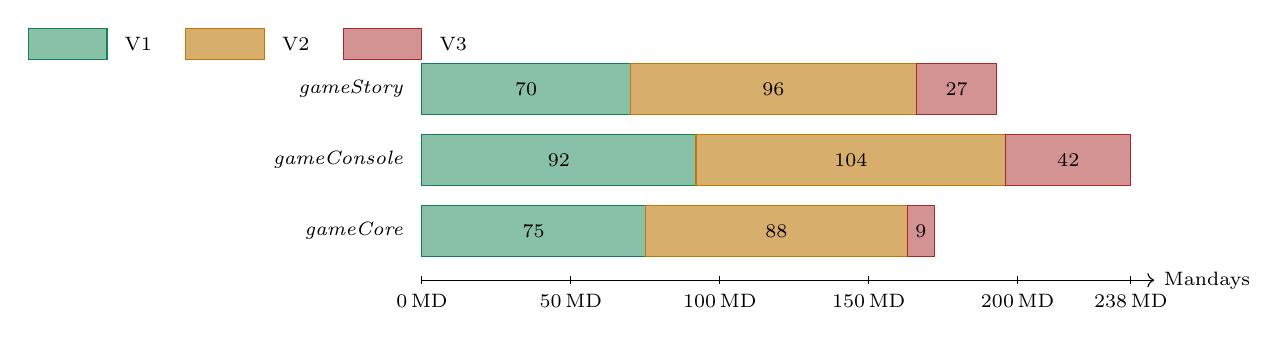
\begin{tikzpicture}[every node/.style={font=\scriptsize}]
% Stacked bar chart showing version contribution per module
\def\totalW{9.0}
\def\barH{0.65}
% Legend
\node[fill=v1green!50,draw=v1green,minimum width=1cm,minimum height=0.4cm] at (-4.5,1.8) {};
\node[right] at (-3.9,1.8) {V1};
\node[fill=v2amber!60,draw=v2amber,minimum width=1cm,minimum height=0.4cm] at (-2.5,1.8) {};
\node[right] at (-1.9,1.8) {V2};
\node[fill=v3red!50,draw=v3red,minimum width=1cm,minimum height=0.4cm] at (-0.5,1.8) {};
\node[right] at (0.1,1.8) {V3};

% gameStory bar: V1=70, V2=96, V3=27 → total=193
% scale: 9cm / 238 (max) = 0.03782
\def\scale{0.03782}
% gameStory row (y=0.9)
\def\ygs{0.9}
\fill[v1green!50,draw=v1green] (0,\ygs) rectangle (70*\scale,\ygs+\barH);
\fill[v2amber!60,draw=v2amber] (70*\scale,\ygs) rectangle (166*\scale,\ygs+\barH);
\fill[v3red!50,draw=v3red] (166*\scale,\ygs) rectangle (193*\scale,\ygs+\barH);
\node[left] at (-0.1,\ygs+\barH/2) {\textit{gameStory}};
\node at (35*\scale,\ygs+\barH/2) {70};
\node at (118*\scale,\ygs+\barH/2) {96};
\node at (179.5*\scale,\ygs+\barH/2) {27};

% gameConsole row (y=0)
\def\ygc{0}
\fill[v1green!50,draw=v1green] (0,\ygc) rectangle (92*\scale,\ygc+\barH);
\fill[v2amber!60,draw=v2amber] (92*\scale,\ygc) rectangle (196*\scale,\ygc+\barH);
\fill[v3red!50,draw=v3red] (196*\scale,\ygc) rectangle (238*\scale,\ygc+\barH);
\node[left] at (-0.1,\ygc+\barH/2) {\textit{gameConsole}};
\node at (46*\scale,\ygc+\barH/2) {92};
\node at (144*\scale,\ygc+\barH/2) {104};
\node at (217*\scale,\ygc+\barH/2) {42};
% gameCore row (y=-0.9)
\def\ygr{-0.9}
\fill[v1green!50,draw=v1green] (0,\ygr) rectangle (75*\scale,\ygr+\barH);
\fill[v2amber!60,draw=v2amber] (75*\scale,\ygr) rectangle (163*\scale,\ygr+\barH);
\fill[v3red!50,draw=v3red] (163*\scale,\ygr) rectangle (172*\scale,\ygr+\barH);
\node[left] at (-0.1,\ygr+\barH/2) {\textit{gameCore}};
\node at (37.5*\scale,\ygr+\barH/2) {75};
\node at (119*\scale,\ygr+\barH/2) {88};
\node at (167.5*\scale,\ygr+\barH/2) {9};
% x-axis labels
\foreach \x in {0,50,100,150,200,238}{
  \draw (\x*\scale,-1.15)--(\x*\scale,-1.25);
  \node[below] at (\x*\scale,-1.25) {\x\,MD};
}
\draw[->] (0,-1.2)--(\totalW+0.3,-1.2) node[right] {Mandays};
\end{tikzpicture}
\end{center}

\subsubsection{Phân Tích theo Pha Phát Triển}

Dựa trên công thức ước tính, công sức được phân bổ tự nhiên qua 5 pha theo tỷ lệ cố định:

\begin{center}
\renewcommand{\arraystretch}{1.35}
\begin{tabularx}{0.96\linewidth}{|l|X|r|r|}
\hline
\rowcolor{headerGray!30}
\textbf{Pha} & \textbf{Mô tả \& Nguồn gốc} & \textbf{MD} & \textbf{\%} \\
\hline
\rowcolor{rowLight}
\textbf{Design} & 0.5\,MD/function (tất cả functions trong components) + 0.5\,MD/fix & 108 & 17.9\% \\
\textbf{Implement} & 1.0\,MD/function (cốt lõi xử lý) + 1.0\,MD/fix & 215 & 35.7\% \\
\rowcolor{rowLight}
\textbf{Test (Unit)} & 0.5\,MD/function (self-testing) + 0.5\,MD/fix & 108 & 17.9\% \\
\textbf{Integrate} & 1.0\,MD/function (cross-component integration, không áp dụng cho fixes độc lập) & 173 & 28.7\% \\
\rowcolor{rowLight}
\textbf{Deploy} & Bao gồm trong Integration (CI/CD, build scripts, WASM) 
& — & — \\
\textbf{Fix / Regression} & Đã được tính trong Independent Fixes (42 issues × 2\,MD) & 84 & $\subset$ above \\
\hline
\rowcolor{headerGray!20}
\textbf{Grand Total} & \textit{Design + Implement + Test + Integrate} & \textbf{603\,MD} & 100\% \\
\hline
\end{tabularx}
\end{center}

\noindent\textit{Lưu ý:} Pha \textbf{Conceptualize} (phân tích yêu cầu, kiến trúc tổng thể) được hoàn thành trước V1 và đã tài liệu hóa trong §03--§07 (SRS + SDS), không tính vào effort development.
Pha \textbf{Fix} bao gồm 42 issues đã ghi nhận (5+9+0 gameStory; 4+10+0 gameConsole; 6+8+0 gameCore) và được tích hợp vào Implement + Test của từng version.
\subsubsection{Phân Tích Phiên Bản \texorpdfstring{$\times$}{x} Pha Phát Triển}

\begin{center}
\renewcommand{\arraystretch}{1.35}
\begin{tabularx}{\linewidth}{|X|r|r|r|r|r|}
\hline
\rowcolor{headerGray!30}
\textbf{Version} & \textbf{Design MD} & \textbf{Implement MD} & \textbf{Test MD} & \textbf{Integrate MD} & \textbf{Total} \\
\hline
\rowcolor{v1green!10}
\textbf{V1} & 34 & 69 & 34 & 69 & \textbf{206} \\
(+Fixes V1) & +7.5 & +15 & +7.5 & — & (+30) \\
\rowcolor{v2amber!10}
\textbf{V2} & 39 & 78 & 39 & 78 & \textbf{234} \\
(+Fixes V2) & +9 & +18 & +9 & — & (+36) \\
\rowcolor{v3red!10}
\textbf{V3} & 11 & 22 & 11 & 22 & \textbf{66} \\
(+Fixes V3) & — & — & — & — & (0) \\
\hline
\rowcolor{headerGray!20}
\textbf{Grand Total} & \textbf{101} & \textbf{202} & \textbf{101} & \textbf{169} & \textbf{573} \\
\textit{incl.\ all fixes} & 
\textbf{108} & \textbf{215} & \textbf{108} & \textbf{169} & \textbf{600$\approx$603} \\
\hline
\end{tabularx}
\end{center}

% ══════════════════════════════════════════════════════════════════
\subsection{Giá Trị Đầu Tư \& Tóm Tắt cho Nhà Đầu Tư}
% ══════════════════════════════════════════════════════════════════

\begin{tabularx}{\linewidth}{|l|X|}
\hline
\rowcolor{headerGray!25}
\multicolumn{2}{|c|}{\textbf{Tổng Hợp Đầu Tư Dự Án cTetris}} \\
\hline
\rowcolor{rowLight}
\textbf{Tổng công sức} & \textbf{603 Mandays} (≈\,4{,}824 giờ kỹ thuật hiệu quả) \\
\textbf{Phân bổ module} & gameConsole 39.5\% (238 MD) · gameStory 32.0\% (193 MD) · gameCore 28.5\% (172 MD) \\
\rowcolor{rowLight}
\textbf{Phân bổ phiên bản} & V1 Foundation 39.3\% (237 MD) · V2 Feature-rich 47.8\% (288 MD) · V3 Cloud 12.9\% (78 MD) \\
\textbf{Số lượng tính năng} & 173 hàm/functions trong components;
42 issues đã giải quyết \\
\rowcolor{rowLight}
\textbf{Nền tảng kỹ thuật} & C++17 · SDL3 · SQLite · Emscripten WASM · Cloudflare D1 · GitHub CI/CD \\
\textbf{Đa nền tảng} & Desktop (macOS / Windows / Linux) + Web (WASM / GitHub Pages) \\
\rowcolor{rowLight}
\textbf{Giá trị cốt lõi} & Module-driven architecture đảm bảo mở rộng độc lập;
Version-driven roadmap minh bạch tiến trình; Phase-driven process kiểm soát chất lượng từng bước \\
\hline
\end{tabularx}

\label{LastPageProjectEffortEstimation}
\end{document}